\documentclass{article}

\usepackage[a4paper, total={15cm, 24.5cm}]{geometry}
\usepackage{float}
\usepackage{graphicx}
\usepackage{amsmath}
\usepackage{array}

\title{Computer Security}
\author{Elia Ravella}
\begin{document}
	\begin{titlepage}
		\maketitle
	\end{titlepage}
	
	\tableofcontents
	\clearpage
	
	\clearpage \part{Introduction} 
		\section{Security}
			What is security? First, we need to distinguish \emph{security} itself and \emph{safety}; the first represents a system that protects from the outside, the second a system that does not harm when it's used.
			
			\subsection{What is a secure system and how to engineer one}
				Famous triangle problem, this time with CIA properties
				\begin{itemize}
					\item Confidentiality: only authorized entities can access information
					\item Integrity: only authorized entities can modify information;
					\item Availabilty: data must be available to all authorized entities in a determined time constraint.
				\end{itemize}
				"You can take only two" problem: A conflicts with C and I.\\
				System security is an engineering problem: it's crucial to find an \emph{optimal tradeoff} between properties to be ensured, and costs to be faced when securing such properties.
			
			\subsection{Entities in a secure system}
				\begin{itemize}
					\item Vulnerability: something that allows to violate one of the CIA properties. It can be something as a design errors, a construction error, or a use defect. Even an \emph{inherent property} of a system can be a vulnerability.
					\item Exploit: a specific way to use a vulnerability (or more) to violate one of CIA properties.
					\item Asset: values of a system, properties that must be protected. Depending on the context a system operates in, different assets can be defined. We should always think about which components are damaged in the case of a successful attack: can be
						\begin{itemize}
							\item the users of a system
							\item the company that produces the system
							\item the physical environment the system is in
							\item also intangible assets, like the \emph{reputation} of the users/owner of the system
						\end{itemize}
					\item Threat: \textbf{possible / potential} violation of CIA constraints. A threat is linked to a threat agent, that's the actual physical person / system that performs the potential attack.
					\item Attack: \textbf{intentional} use of an exploit to violate CIA properties.
					\item Risks: combination of assets, vulnerabilities and threats. Formally (using economic value) they're A*V*T. Risk management takes care of the first two properties. The security problem is to manage the reduction of vulnerabilities and the recovery / mitigation plan. 
				\end{itemize}
				\textbf{A vulnerability can be present without any exploits. An exploit depends from a set of vulnerabilities}.\\
				
				\paragraph{Security vs Cost Balance}
					As usual, costs can be separated in direct and indirect costs. In this scenario, direct costs are related to the actual put-in-place of a solution. Indirect costs, instead, are all the user experience costs, all those experience-heaving procedures, for example. So EVERY SINGLE SECURITY SOLUTION ADDS A COST.
					
				\paragraph{Trust and Boundaries}
					The security problem must have boundaries, otherwise it will cover over the universe. So, subparts must become \emph{trusted} and be \emph{assumed secure}. All the system that are beyond (below) the boundary are assumed secure too. The trusted element is the one to be tested most. 
			
	\clearpage \part{Cryptography}
		\section{Cryptography, cryptoanalisys, cryptology}
			Cryptography is the building of secure mathematical systems. Cryptoanalisys is the discipline of analyzing such systems, and trying to break them. Cryptology is the union of both.\\
			Cryptography \emph{as a discipline} was formalized by Claude Shannon in 1949. The (still actual) formalization of a cryptosystem is composed of 3 main components:
			\begin{enumerate}
				\item the \emph{plaintext}, the message to be encoded
				\item the reversible encoding function, which usually depends on a \emph{key}
				\item the \emph{cyphertext}, the encoded message
			\end{enumerate}
			
			\subsection{Confidentiality and Integrity}
				"Why a cryptosystem"? The two main features that a cryptosystem must have are
				\begin{enumerate}
					\item confidentiality: only the recipients can read and utilize the information in the message.
					\item integrity: data can't be altered in the message passing. If so, the recipient can detect the change.
				\end{enumerate}
				The Kerchoff's principles states that the security of a cryptosystem relies \emph{solely} on the secrecy of the key, rather than the secrecy of the algorithm. The algorithm itself, in fact, should remain public. This means that a secure system is \emph{transparent} inherently.\\
				\textbf{The key must be the trusted element of the entire cryptographic system}.\\
				Formally, a perfect cypher does not leak any information about the message if and only of
				\begin{equation}
					P(M=m \,\vert\, C=c) = P(M=m)
				\end{equation}
				As theorized by Shannon. So "the probability of observing message m given cypher c is indipendent from the cyphertext given". Shannon also proved that perfect cyphers exists: they're \emph{one time non reusable key systems, with the lenght of the key equal to the lenght of the message} (also known as the \textbf{Shannon Theorem)}.\\
				The only perfect cypher implementation is OTP, One Time Pad. Classic XOR based encryption with a one time password (pre shared) that is long as the message. The cool thing about perfect cyphers such as OTP is that bruteforcing the cyphertext simply returns all the possible combination of plaintext, rendering so useless the brutaforce approach.
			
			\subsection{Cryptoanalysis}
				All the "brutaforce" fuss is about the problem of determining "how much a system is breakable". Bruteforce "always works", but it's a costly approach. So, it formally represents an \emph{upper bound} to the deciphering provedure complexity for that cypher. Other (more smart) attacks are 
				\begin{itemize}
					\item Cyphertext attack - only cyphered text are available, a key/algorithm leak of information must be exploited
					\item Known plaintext attack - comparation between the plain and crypted texts should lead to the key
					\item Chosen plaintext attack - reverse engineering of the algorithm
				\end{itemize}
				distinguished by the materials available to the attacker, and orderd in increasing complexity.
				
			\subsection{Remarks on Cryptosystems}
				\begin{enumerate}
					\item Security of a CS is based on the robustness of the \emph{algorithm}
					\item No algorithm is invulnerable to brute force attacks, exception made for \emph{one time pads}
					\item An algorithm is said to be broken if there's at least one way \emph{faster than bruteforce} to bypass it
					\item The only way to prove a cypher is robust is to try to break it
				\end{enumerate}
		
		\section{Symmetric Encryption}
			Classic: Alice uses key K to encrypt message M into cypher C, then Bob uses the very same key K to decipher cypher C into message M. Problem: exchanging keys. We need a \emph{trusted separated channel} to exchange the key. What is a trusted channel? It generally is a different channel that both the recipients \emph{consider trusted} and generally \emph{requires a different attack to be violated}.\\
			We so must try to find a way to send to all recipents the key \emph{in a secure way}. Another issue with symmetric encrypted communication is scalability, each pair of user in a network should have a unique key. 
			
			\subsection{How to build a secure symmetric system}
				Three characteristics are fundamental to ensure the robustness of a symmetric cypher:
				\begin{enumerate}
					\item \emph{Substitution}: replacing bytes. Ceasar's cypher is the perfect example of only-transposing symmetric cypher.
					\item \emph{Transposition}: also called diffusion, it consists of "swapping the value of bits", messing with the order in which the plaintext is translated.
					\item \emph{Multi Alphabetical Cyphers}: to mask structure and repetition in the plaintext several target alphabets can be (must be) used at the same time.
				\end{enumerate}
				
				\paragraph{Keyspace}
					With keyspace is intended the \emph{set of possible keys}. There's an exponential correlation between the size (rank) of this set and the temporal complexity of the brutaforce effort. This means that more possible keys (generally translated in "how many bits is the key made of") more the time needed to bruteforce the cypher. \emph{This is valid in the current silicon architecture computers. Quantum computations could change this}.
		
		\section{Asymmetric Encryption}
			Cyphers with \emph{two} directional keys instead of one. What is encrypted with key A can be decrypted \emph{\textbf{only}} with key B and viceversa. What you can't do is
			\begin{itemize}
				\item decrypt the message with the \emph{same} key you used to encrypt the message
				\item deduce (calculate) one key from another
			\end{itemize}
			This approach enables "public key scenarios" due to the asymmetricity of the encryption mechanism. The robustness of this methods relies on the function used to encrypt the plaintext, that must be easy to apply \emph{but difficult to reverse}.\\
			To make a public key scenario works we must add to the set of trusted elements (that contains the private keys) a \emph{trusted assumption}: "only Bob knows Bob's private keys".\\
			In asymmetric encryption the key lenght is an important measure of safeness. However, while in symmetric cypher the lenght of the key measure the number of decription attempts, in asymmetric cypher it measures the \emph{number of key-breaking attempts}. That implies that asymmetric cyphers are "easier" to crack because of the approach chosen to encrypt. This also means that asymmetric and symmetric cyphers cannot be compared only using the key lenght.
			
			\subsection{Hash Functions}
				A hash function is a function that maps an \emph{arbitrary lenght string} in input on a \emph{fixed lenght string} at the output. Usually, input strings lenght are much longer than output ones $\Rightarrow$ \emph{collisions}. A good hash function satisfies three properties:
				\begin{enumerate}
					\item preimage attack resistance: the function is \emph{hard to invert}.
					\item second preimage attack resistance: it must be difficult to find a input string that have the same hash to another one \emph{given} (if the function is not preimage resistant it's not second preimage resistant too. The opposite is not true tho).
					\item collision resistance: it must be hard to find 2 inputs with the same output.
				\end{enumerate}
				
				\subsubsection{Attacks to Hash Functions}
					Hash function may be broken. This means that it's possible to find the original text from the cyphertext \emph{faster than bruteforcing}, just as the definition of broken cryptosystem. Two methods are used to attack a hash function:
					
					\paragraph{Arbitrary Collision}
						This is a first/second preimage attack: the attacker tries to deduce $x \,\vert\, H(x) = h$ or, respectively, $y \,\vert\, y \neq x \wedge H(x) = H(y)$.\\
						Again, an hash function is broken if this can be completed \emph{faster than bruteforcing it}.
						
					\paragraph{Simplified Collision Attack}
						Exactly the same approach as the arbitrary collision attack, but exploiting some probabilistic aspects of the collision (birthday paradox).
				
				\subsubsection{Digital Signature}
					Classic digital signature mechanism: an hash function produces a digest of a document, that's then encrypted with the private key of the sender. The receiver (to both check for identity of the sender and the integrity of the document) does the same: hashes the document and produces a digest, that's then compared with the decrypted version of the received one.\\
					A big issue in this case is "who to trust". To estabilish a list of trusted elements the current infrastructure relies on Certification Authorities, a tree-like structure (a hierarchical group) of entities that each signs with a trusted key (a trusted role) the certificates.
			
	\clearpage \part{Authentication}
		\section{Identification and Authentication}
			What's the difference between identification and authentication? The first represents the act of "telling your identity". Authentication means to \emph{proof} the stated identity. Authentication must be \emph{bidirectional} or \emph{mutual}: both entities must acknowledge each other identity and the proof.
			
			\subsection{Authentication factors}
				To identify someone, three methods can be used:
				\begin{enumerate}
					\item Authentication by "to know" factor (passwords, pins)
					\item Authentication by "to have" factor (cards, ids)
					\item Authentication by "to be" factor (fingerprint, voice)
				\end{enumerate}
				Multi factor authentication uses more than one factor to authenticate.
				
				\subsubsection{To Know Authentication}
					To Know authentication systems relies on something the user willing to authenticate remembers, or is supposed to know. These systems are low cost, are easy to deploy and easy to use (due to the spread of such systems). Systems basing on to know auth are systems that rely on passwords, pins, login data combination etc.\\
					On the other hand, the secrets the user is asked to keep can be easily stolen or guessed, or even cracked (bruteforced). 
					
					\paragraph{Countermeasure Against Password Wearing}
						Three different attacks can moved against a passwrod-secured system, each one has a valid countermeasure:
						\begin{enumerate}
							\item against snooping, it's valid to change password often;
							\item against cracking, it's useful to enforce complexity of the password;
							\item against guessing, it's useful to ask for a nonsense password, or at least not easy to pin to the user;
						\end{enumerate}
						A system cannot put in place all these countermeasure, because they are \emph{costly}: they heavy the use of a system (a system that asks for a 64 mixed characters every 2 days).
						
					\paragraph{Secure Password Exchange, Challenge Response}
						Authentication phase, exchange of messages between two entities A and B that mutually authenticate each other
						\begin{enumerate}
							\item A to B: This is my identity. Let me authenticate
							\item B to A: nice. Compute hash(random-data + secret) + random-data
							\item A to B: hash(random-data + secret)
							\item A to B: nice. Compute hash(random-shit + secret) + random-shit
							\item B to A: hash(random-data + secret + random-shit)
						\end{enumerate}
						Where secret is the password, generally. The supposition is that both entities \emph{know} the secret.
						
					\paragraph{Secure Password Storage}
						Passwords are the secret upon it's based the security of a system (an authenticating one, at least). How to enforce password security?\\
						To protect a file (data in general) the techniques are always the same: 
						\begin{itemize}
							\item Encyption
							\item Salting (modifying stored passwords to mitigate dictionary attack)
							\item Access Control
							\item Password Recovery procedures that not disclose sensitive infos
						\end{itemize}
				
				\subsubsection{To Have Authentication}
					To Have factor relies on \emph{a phisycal device / object} that must be associated to a person willing to authenticate. The problem remains the human factor: this time the security of the system depends on how the key (secret) is handled by the person associated to it.\\
					In any case, to have authentication system are low cost and offer a good level of security. On the other hand, they're hard to deploy, and the tokens / cards are easy to be lost or destroyed / compromised.
				
				\subsubsection{To Be Authentication}
					To be authentication asks the person willing to authenticate to prove to be who s/he declares to be by biometrically satisfy a costraint (like having a certain fingerprint, hand geometry, iris pattern...).\\
					Although this kind of authentication is very effective (it's \emph{really} difficult to emulate someone else's fingerprint) the list of disadvantages for biometric security systems is quite long:
					\begin{enumerate}
						\item They're hard to deploy and set up. Moreover, usually during the setup phase an invasive test must be performed
						\item The matching of the feature selected is non-deterministic: accepting or rejecting a person depends on a threshold of accuracy, and this can act differently from time to time
						\item They're not \emph{entirely} secure: a fingerprint can be cloned
						\item Biometric features \emph{change} over time
						\item Privacy issues: people \emph{may not want} to distribute personal features involved in a biometric security system
					\end{enumerate}
				
				\subsubsection{Single Sign On}
					Single sign on was proposed as a countermeasure to password reusing. This system is based on a 1-2 factors authentication and \emph{a single trusted host}. This is simply the "delegating authentication to someone else" method of authentication, the \emph{external auth} method. Two main approaches:
					\begin{itemize}
						\item SAML approach: an external service serves as authentication factor
						\item OAuth approach: the external service \emph{just helps the authentication}, giving the user a code in order to sign on to the principal service
					\end{itemize}
					This is also complicated to implement: an app should (in order to implement OAuth or SAML) complicate a lot its flow of usage (user experience) in order to just authenticate a user.\\
					Moreover, the trusted factor is a SPOF.
					
		\section{Access Control}
			Access control is all the protocols and procedures that \emph{allow or deny} certain operations to be applied on certain resources. This operation is usually performed by a reference monitor, that carries out the verification of the rules and the roles (lol).
			
			\subsection{Discretionary Access Control}
				The resource owner assigns the priviledges to users. It's the most standard access control system: for every user (or entity) a set of permissions is defined that describe the rights of each one. A DAC is defined by 3 set of entities:
				\begin{enumerate}
					\item subjects: the actors, the users
					\item objects: the resources
					\item actions: the actions that subjects can perform on objects, that are restricted by the rules
				\end{enumerate}
				The reference monitor organizes the subjects and the objects in a two entry map that lists what every user can do to each resource. This implementation is called HRU model, due to its designers. What this model also allow is to check if the access control system works as intended: if it can be proven that a user can "upgrade" his permissions \emph{on his own} the system is unsafe by design. This is an undecidable problem btw.\\
				This implementation (let alone the scaling problem) is a little bit difficult to utilize, so alternative implementations are possible, like:
				\begin{itemize}
					\item Authorization tables: DBMS like approach, it's a HRU model with not null entries
					\item Access control lists: used in networking, each objects records his own owners/users
					\item Capability list: each user "remembers" the authorization he got
				\end{itemize}
				See how the last two implementations are just "read the HRU table coloumn by coloumn" and "read the HRU table row by row".
				
			
			\subsection{Mandatory Access Control}
				Clearance / Sensitivity access control management. Based on user's roles combined with "objects' secrecy levels". The idea behind is: do not let users assign priviledges. The priviledges are set by an administrator, that assigns levels to users and to resources. Each user level can access only a subset of the resource level. This is usually combined with a labeling system that categorizes in a finer way the resources, orthogonally to the secrecy level.\\
				Then, read/write accesses are granted as rules, for example
				\begin{itemize}
					\item No read up
					\item No write down
				\end{itemize}
			
			\subsection{Role Based Access Control}
				RBAC is kinda a hybrid of DAC and MAC, and can also enforce them: if configured in the right way, it can act as a DAC or as a MAC. The idea is similar to the one that driven MAC design ("no self assigning dynamic priviledges") but the roles are no more structured in a rigid hierarchy but instead are simply \emph{a label to a set of priviledges}.
					
	\clearpage \part{Software Security}		
		\section{What is software security?}
			With "software security" is intended the meeting of the non-functional requirement (obviously for a software) of \emph{being secure}. This is often overlooked in the process of software developing, but to remind the importance of this non functional requirement, it's sufficient to think about the name of the unmet security specifications: \textbf{vulnerability}.\\
			Recap on definitions:
			\begin{itemize}
				\item Vulnerability: fault in the target software/system
				\item Exploit: method to leverage a vulnerability to harm a system
			\end{itemize}
			
			\paragraph{Vulnerability / Attack relationship}
				\begin{figure}[H]
					\centering
					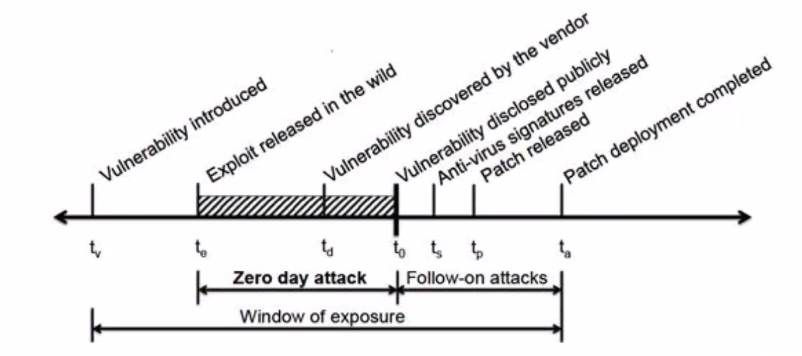
\includegraphics[width = \textwidth]{./images/vulLifeCycle.png}
				\end{figure}
				This graph explains how the vulnerability life cycle interacts with the actual attacks cycle to a software. To be noted:
				\begin{itemize}
					\item zero days attacks happens when the vulnerability is "out in the wild", known only to hackers
					\item at the moment the vulnerability is \emph{exposed to the public} other security firms can start working on side solutions to limit attacks, weakening the actual attackers margin
					\item the window of exposure is closed \emph{ONLY} after the patch is installed \emph{everywhere}
				\end{itemize}
				
		\section{Principles of Secure Design}
			We can define a list of principles, guidelines, to create a secure software:
			\begin{itemize}
				\item Reduce the privileged parts to the minimum to avoid permissions vulnerability windows
				\item KISS principle, reduce the complexity of a software
				\item Avoid shared resources, or unsafe external libraries. Use instead safe and known secure libraries
				\item Default deny principle: allow only authorized operations
				\item Use filters on input and output
			\end{itemize}
			
		\section{Vulnerabilities}
			\subsection{Buffer Overflow}
				Memory vulnerability, one of the most famous technique to exploit a software. Practically, it means that a piece of data is inserted in a buffer that is smaller then the data itself. This enables the attacker to overwrite "sensitive" portion of the memory, and (in the worst case) inject malicious code. The thing that makes buffer overflow so dangerous is the way a buffer is allocated in 99\% of cases, so calling a function that does that: this allows the attacker to \emph{directly overwrite the return address from that function}.
					
				\subsubsection{Buffer Overflow Defense}
					Defending against buffer overflow means defending against a super powerful type of vulnerabilities that can harm a whole software. This kind of defense can be put in place in three main regions:
					
					\paragraph{Source Code Level}
						The source code is where the vulnerabilities is rooted. Making the source code safe from potential buffer overflow means \emph{educating developers} and \emph{using safe libraries} or safe version of already written libraries. The technology stack should be secure too!
						
					\paragraph{Compiler Level}
						The compiler can inform the developer of the possible vulnerabilities, but this measure still rely on the human. Another approach is to change the order (randomizing) of the arguments onto the stack. \emph{BUT} this is only temporary, as the buffer overflow is still there and can be found by exploiters by analyzing the output of the compiler, the binaries.\\
						The "canary mechanism" is also used: a spy is put on top of the stack (the canary is put by the prologue of the function) and then verified by the epilogue. If the canary is different, then the function has been overflowed, and the program has been compromised. Multiple approaches can be applied to canaries:
						\begin{itemize}
							\item Random-per-run canaries: each run of the program the canary is changed
							\item XORandom canaries: the value of the canary is obtained \emph{from the data it's trying to protect}, preventing further unwanted memory modification
							\item Terminator canaries: the canary is entirely made up of terminator characters (so cannot be stringcopied)
						\end{itemize}
						
					\paragraph{OS Level}
						The OS has two main mitigation that can use:
						\begin{itemize}
							\item Non executable stack, so flagging some portion of the memory as data-only. This does not mitigate the "return to a function" type of attacks.
							\item Address space layout randomization: scrambling the memory pages layout. This renders quasi-impossible guessing rightly the return address.
						\end{itemize}
						
			\subsection{Format String}
				Format string vulnerabilities creep out near printing function, when these are "badly formatted": no format (or a wrong one) is provided to print the parameters. Classical example: passing a placeholders-only string to a printf without formatting will print the content of the memory filling that placeholder, \emph{disclosing information}.
				
				\subsubsection{Exploiting Format String Bug in a ANSI C Program}
					We have several placeholders and placeholders extensions we can use to make a format string vulnerability super dangerous.\\
					Placeholders:
					\begin{enumerate}
						\item \%d and \%i to print integers
						\item \%u to print unsigned decimals
						\item \%X and \%x to print unsigned hexadecimals
						\item \%o for octals
						\item \%c for chars, \%s for strings
					\end{enumerate}
					Placeholder modifiers (of interest):
					\begin{enumerate}
						\item N\$: if inserted between the \% and the placeholder character tells the formatter to go to the N-th parameter.
						\item \%n: this placeholder \emph{writes the number of chars printed} so far to the address pointed \emph{by the argument}. The important thing is: whatever value is in the memory \emph{where the argument is searched}, it will be interpeted as a memory location. We will also use his brother \%hn, that writes a shortint.
						\item also, the \%c placeholders for chars can be extended as \%Nc where N is the number of times the first char argument must be prented.
					\end{enumerate}
					So, how do we exploit this?\\
					First of all, we can build a "memory scanner" with just "\%N\$x" and iterating over N: this will print the hexadecimal code of all the "arguments" (memory slots) after the one passed as an argument. Remember, we're sure to be on the stack of the application, because this bug targets \emph{printing functions}, and the exploit string will be the parameter of such function. This is already a vulnerability: we can exploit this to make tha pplication leak information by \emph{directly accessing its memory space}.\\
					To also write, obviously we need to use \%n. We must combine the character-generating placeholder \%Nc and the target-sniping placeholder N\$ in order to obtain the right alignement of the memory and to write \emph{exactly there}. This also highlights the main difference between a buffer overflow vulnerabilty and a format string one: while the BOF acts as a tank overwriting all the memory it traveses, the format string modify exactly the portion of memory needed, leaving the rest unchanged. 
					
				\subsubsection{Format String Defence}
					Being another memory vulnerability, many of the solutions explained for the buffer overflow are still valid. Being the format string dependant strictly on some printing functions, it can be easily patched by modifying this very functions (indeed, a secure version of libc exists). Moreover, compilers have learnt to detect "unsafe calls" to printing functions and signal them.
					
			\subsection{Final Remarks on Vulnerabilities}
				The two vulnerabilities we've seen (format string and buffer overflow) are two common memory vulnerabilities that can be exploited to manipulate the behaviour of a system, tricking it into leaking information or worse, like executing malicious piece of software. These kind of vulnerabilities all originate from a "irresponsible" programmer that does not have in mind how a software can be exploited; however, against these vulnerabilities several countermeasures can be taken and put in place, and many of those eventually finish embedded in operating systems. What's more important is to consider safety a semi-functional requirements for software.

	\clearpage \part{Web Security}
		\section{What is Web Security?}
			The main difference between a "traditional" software attack and a web attack is often only the exposure of the app itself. This is also the motivation that renders the web attacks so impactful and web vulnerabilities so crucial to solve.
			
			\subsection{Architectural View of an Attack}
				Let's talk about the classic 3 tiered architecture:
				\begin{enumerate}
					\item Client and presentation layer
					\item Controller layer
					\item Persistence / Data layer
				\end{enumerate}
				HTTP connects the first two layers (and often also the two back ones). The statelessness of HTTP is also the major securty issue: it provides \emph{determinism} in the behaviour of the web applications. Also, it's text based; easy to counterfeit. 
				
				\subsubsection{The Untrustworthy Client}
					The client is the only piece of software that the attacker can use, most of the times. The golden rule for web programming is to assume that \emph{all clients are attackers}, and thus give that part of the software the minimum power\footnote{With \emph{power} in this case is meant "possibility to harm". This usually translates in limiting as much as possible the client actions and doublecheck server side all the data that comes from them.} possible.
				
		\section{Filtering}
			Filtering is the first line of defence wrt any kind of attack. It's obvious: if an attacker \emph{cannot add malicious stuff} or \emph{cannot even access dangerous services} it cannot harm. BUT filtering is hard: what do you filter? What do you blacklist? This is the classic filter system build:
			\begin{enumerate}
				\item Start with a whitelist approach (deny all except allowed)
				\item Proceed "a regime" with a blacklist method (deny bad people)
				\item Perform \emph{escaping}, so neutralize possible malicious inputs. This procedure is often referred to as "hygienizing input"
			\end{enumerate}
			Filtering also comes into play when it's time to separate the data from the executables: when the data can be executed, when it's just data?
			
			\subsection{Filtering Problems: Cross Site Scripting}
				Cross Site Scripting (XSS) is a kind of attack that just occurs when \emph{data is not differentiated enough from code}. MSN allowed you to enter HTML an JS code into comments, but a JS-written comment will \emph{executed by all the people that visit that page}. We can distinguish three type of XSS: Stored, Reflected and DOM-based XSSs.
				
				\paragraph{Stored XSS}
					The MSN example. The attacker can memorize malicious code in the server and this is then propagated to other clients. This happens if the malicious code is not recognized as such; all the clients that download the malicious resource find valid code to be executed, and blindly execute it.
					
				\paragraph{Reflected XSS}
					Reflected XSS does not rely on the server \emph{to memorize the exploit}: the attacker usually craft a malicious packet (or request) and sends it directly to the victim. This request will \emph{trigger an existing vulnerability} in a site (that can also be totally unaware of it). The classic attack of this kind exploits a site that \emph{does not hygienize the content it receives through a GET} and presents it as-is to the user; for the attacker it's enough to craft an ad-hoc request and have the user trigger it (mail attack).
				
				\paragraph{DOM based XSS}
					DOM based attacks are similar to reflected attacks (in fact, the idea is the same; often also the implementation). The main difference is that the server is completely cut off from the attack: the reflection of the malicious code is handled by the \emph{client side code} such as javascript scripts built in pages. The target page (the one that in classical reflected attacks actually \emph{hosts a vulnerability}) now can be totally embedded in the request. These kind of attacks are just pumped up reflected XSS attacks.
					
				\paragraph{XSS is Powerful}
					JavaScript and other web scripting languages used in dynamic pages are built and executed with the client golden rule in mind: \emph{do not trust clients}. This does not mean that they cannot harm: they have access to personal information such as cookies, the session storage (and often the LocalStorage too) and they can perform \textbf{drive by downloads}\footnote{just issuing a download "fraudolently", that sends malicious code to the client.}.
				
			\subsection{Same Origin / Content Security Policy}
				\paragraph{Same Origin Policy}
					SOP is a principle implemented in all web clients, that enforces the "don't touch other's stuff" rule: all client side code loaded from origin A can access only to resources loaded from origin A. This simple policy can be bypassed in several ways, and the modern web programming paradigms are making circumventing this rule easier to attackers: it's not so rare that more sites share the local resources (in order to offer enhanced services) or that client side extensions inhibits some of the security countermeasures of the browser itself.\\
				
				\paragraph{Content Security Policy}
					CSP\footnote{https://en.wikipedia.org/wiki/Content\_Security\_Policy}, instead, is a measure adopted \emph{by websites} that aims to mitigate XSS and other code injection attack by \emph{informing the web browser which are the secure contents} that can be trusted\footnote{so, loaded and executed} on that page. It's embedded in the HTTP headers of the response. The CSP is implemented by the majority of commercial browsers. CSP is a great mitigation for attacks, but:
					\begin{enumerate}
						\item writing the policies must be done by hand, and it's difficult
						\item policies must be kept up to date
						\item how many policies are enough? how many break functionalities (for example getting in the way of the loading of a library)?
						\item how does CSP realate with browser extension? (same problem of SOP)
					\end{enumerate}
					Reminder: if a browser does not support / has implemented CSP handling, it cannot use it. (This is to say that CSP is just a specification, and browsers need to implement it).

		\section{Vulnerabilities and Attacks}
			\subsection{SQL Injection}
				Code injection attacks works all at the same way: they add (and then try to execute, or havo other execute it) malicious instructions in a place where these should not be, in order to harm a system. SQL injection is no different: the target this time are not-sanitized input fields in web forms,
				
				\subsubsection{Exploiting a Non Sanitized Form}
					SQL injection is quite easy to understand: take for example a login form, for a newsletter, social network or service that is. The two basic fields to fill are username and password, and will be likely be inserted in a "users" table. \emph{If there's no filter to the input}, I can insert something like " username ';-- " in the username field. This will 
					\begin{enumerate}
						\item Close the string with the character '
						\item Close the query with the character ;
						\item comment the rest of the query with --
					\end{enumerate}
					If the system is simple enough to allow users in the system as soon as this query returns a value then I've successfully logged in withough a password!\\
					Different attack can be performed: instead of commenting, I can inject an always-true condition in order to bypass the password checking (such as OR 1=1) or completely bypass the query system with a UNION attack: some DBMS actually consent to use set operators as UNION, INTERSECTION to filter query results, and this can be exploited by attackers to validate false information.
					
			\subsection{URL Tampering}
				Another surface that's often vulnerable to attacks is the URL of the app we're using. For most web applications the URL is also a string the \emph{encodes the state of the application}, maybe even specifying the exact location (on the \textbf{server}) of the document displayed (this is valid for old directory-structured sites, but it's also true for complex modern applications with explicit parameters in the URL). 
				
				\subsubsection{Path Traversal Attack}
					For old fashioned sites that are just HTML documents collection, the URL is the path on the server that identifies the desired page/document displayed. Again, if \emph{no filter} is present on the URL, nobody can stop an attacker to navigate through the filesystem of the server just by tampering the URL. 
	
			\subsection{Cookies!}
				Cookies were born to help web sites build a user experience that was tailored to the \emph{single client}. The abuse of the cookies (as nowadays web) renders them a weapon of mass surveillance: every action can be stored in a cookie on the client and then accessed to model the client behaviour.
				
				\subsubsection{Cookies for Session Management}
					Cookies are used to store information about the HTTP \emph{session}, a technique used by websites to keep track of the state of an interaction with a client. For example, to keep conversational data about a client, the server can generate a SessionID that than stores as a cookie on the client to identify it, and the data associated to it.\\
					OBVIOUSLY these session tokens should be crafted in a way to not be exploitable:
					\begin{itemize}
						\item if used for authentication, not storing plaintext sensible data
						\item if used for session identification they should not be "predictable"
						\item they should have a clear (and near) expiration date that ALSO should not coincide with the cookie one
					\end{itemize}
					All these things must be kept in mind when designing session interaction in order to avoid impersonating attacks: if an attacker is able to spoof sensitive infos from the cookies he can easily impersonate someone else. 
				
				\subsubsection{Cross Site Request Forgery}
					Forces an user to execute unwanted actions (\underline{state-changing action}) on a web application in which he or she is currently authenticated with ambient credentials (e.g., with cookies).\\
					So, this formal definition states that a CSRF exploits the \emph{client ambient credentials} to fake a set of action to perform on a site.\\
					The classic CSRF attack can be carried out in 4 steps:
					\begin{enumerate}
						\item The victim signs in on a website that (for example) takes information from the client through a form that \emph{exploits ambient variables}.
						\item The victim visits a malicious site (or clicks on a link)
						\item The malicious site generates a fake request (following the form example, a well-crafted POST HTTP request is enough) and with XSS techniques make it execute on the victim web client
						\item This way, the web client executes a malicious web request that \emph{fills out the original form} and it's able to get through because the original website uses the \emph{ambient variables} to authenticate the user
					\end{enumerate}
					
					\begin{figure}[H]
						\centering
						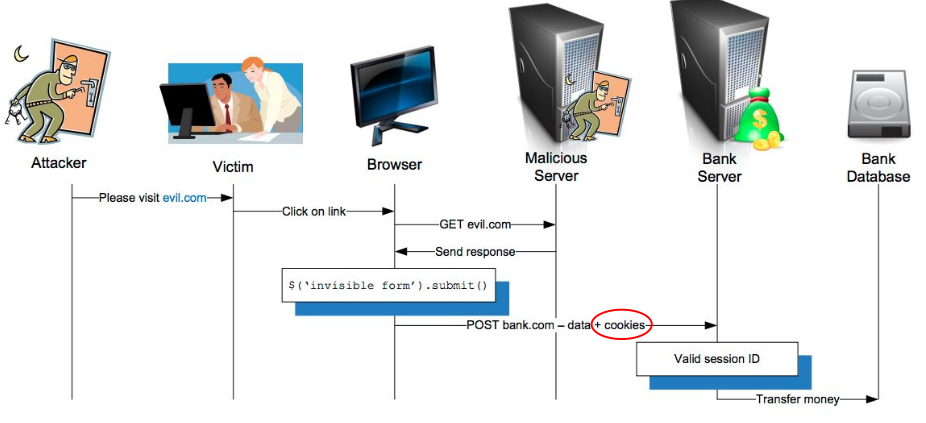
\includegraphics[width = \textwidth]{./images/CSRF1.png}
						\caption{Sequence diagram for a CSRF attack.}
					\end{figure}
					
					\paragraph{CSRF Mitigation Techniques}
						A first form of mitigation for this kinds of attacks is the CSRF token: a set of \emph{random challenge} tokens that are \emph{associated to the user's session} that are \underline{regenerated at each request}. These tokens are sent from the client to the server (but are not stored in the cookies) and the requests are "confirmed" only if the tokens (client-sent and server stored) match. This technique is called \emph{synchronizer token pattern}.\\\\
						Another possible mitigation is the "Same Site Cookies" policy: from Wikipedia, "An additional 'SameSite' attribute can be included when the server sets a cookie, instructing the browser on whether to attach the cookie to cross-site requests. If this attribute is set to 'strict', then the cookie will only be sent on same-site requests, making CSRF ineffective. However, this requires the browser to recognise and correctly implement the attribute, and also requires the cookie to have the 'Secure' flag."
	 
	\clearpage \part{Transport Layer Vulnerabilities and Attacks}
		\section{Security at Network Layer}
			In the internetworking scenario, the attacks are usually put in place targetting design issues of communication protocols, as UDP or TCP. These protocols are not "theoretically" vulnerable, but in order to work they expose information that can be used in a malicious way. Three kinds of attacks are studied in literature:
			\begin{itemize}
				\item Denial of Service (attack to availability)
				\item Sniffing (attack to confidentiality)
				\item Spoofing (attack to integrity and authenticity)
			\end{itemize}
			
		\section{Denial of Service Attacks}
			DoS attacks threaten the availability of an app or service. This can be done in multiple ways, depending on the level that is being attacked (the attacker can deny a service directly on the user's client, deny the access to the communication infrastructure that links client and service or directly making the service unavailable) or the kind of attack carried out.
			
			\subsection{Killer Packets}
				\subsubsection{Ping o Death}
					Killer packets attacks leverages errors is the \emph{protocol implementation} on certain OSs. The classic attack of this kind is the so called "ping of death": a pathological ICMP packet (pathological because "too large") that overflows the receiver buffer, causing it to crash. 
				
				\subsubsection{Teardrop}
					Teardrop attacks exploits a vulnerability hidden in TCP packets, the possibility to specify the offset of the data segment of a fragmented packet\footnote{a TCP feature that enables splitting a network packet into multiple packets} in an inchoerent way, like overlapping packets. This makes impossible to reconstruct the original long packet, making the kernel hang or crash. 
					
				\subsubsection{Land Attack}
					Little bit of history of hacking: Win95 was vulnerable to a particular type of attack that simply consists in crafting an IP packet with the source address equal to the destination address.
					
			\subsection{Flooding}
				Flooding a network means saturate it with requests, above the bandwidth that the infrastructure can hold and manage. 
				
				\subsubsection{SYN flood}
					SYN flood attacks exploits the way a three-way-handshake (the TCP method for estabilishing a connection) is designed. The server \emph{must hold the information} about all clients he's waiting an ack from. So, an attacker can saturate the server by never sending these. The attacker must use different IP addresses to do this (easy enough: a handful of seconds of spoofing gives you the most frequent IP addresses used on a network). This can be easily mitigated by moving the actor that holds the SYN information (storing a SYNcookie, of sorts).
					
			\subsection{Distributed Denial of Service}
				Oppositely to the DoS classic attacks, DDoS attacks exploits a big infrastructure (such as a botnet) to saturate a network/infrastructure/service. The idea remains basically the same as the flooding attacks, but this time the "power factor" is the dimension of the attacker network instead of the use of the resources of the server. Notice how these attacks are \emph{far more difficult to mitigate} because if the hacker can put together a large enough attacking infrastructure there's no way to stop it.\\
				The attacker can either use a network of computers at his disposal (botnets or C\&C infrastructures) or leverage an existing network, as the Smurf attack:
				
				\paragraph{Smurf Attack}
					If the attacker can spoof the victim address (whichever address it may be) it can use it on a network for simply issuing an echo request with at "sender" the spoofed victim address. All the networks echo replies will be redirected to the victims, flooding it. This is a table that calculates the so called \emph{amplification factor} for each protocol.
					\begin{figure}[H]
						\centering
						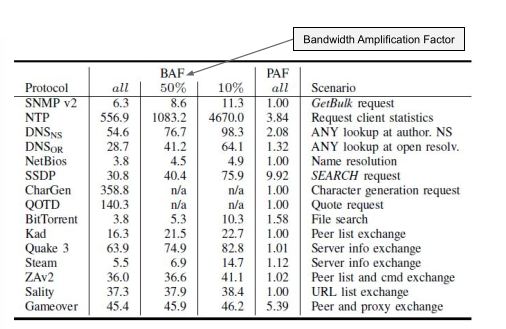
\includegraphics[width = \textwidth]{./images/SmurfAttack.png}
						\caption{The bandwidth amplification factor (BAF) computes the bandwidth multiplier in terms of number of UDP payload bytes that an amplifier sends to answer a request, compared to the number of UDP payload bytes of the request.}
					\end{figure}
					
		\section{Sniffing}
			Sniffing is more a "hearing what's not destinated to you" kind of attack. It's a passive kind of attacks that aims only to retrieve information.
		
		\section{Spoofing}
			\subsection{ARP Spoofing}
				ARP is the protocol that converts IP addresses into lower level adddresses. To be fast (it's deisgned to be only fast) it's unauthenticated, with belief that authentication is done at higher levels. ARP just provides a request response broadcast service in a LAN to do this linking of addresses. ARP spoofing is rather easy: if an attacker detect an ARP request he can send a malicious ARP response in order to \emph{deviate traffic} to another direction, or just interrupt it. This kind of attacks are usually called "ARP poison" attacks.  
				
			\subsection{IP Spoofing}
				The IP source address is not authenticated. This render the IP protocol extremely vulnerable to spoofing attacks. An attacker can spoof an address and use it as the source address in an UDP or ICMP packet. However, he won't be able to receive the responses! He can still sniff them tho...\\
				For TCP protocol (due to the way the sequencing and the handshake are organized) things change. If the attacker can guess the InitialSequence Number he can \emph{blindly complete} a three way handshake, but here's the difficult part: guessing the semi random number chosen by the victim. This is quite difficult now but TCP sequence numbers were chosen with a very low randomness back in the 90s.\\
				Where's the danger? \emph{Man in the middle} attack. A fully impersonating attack, the hacker can fake himself to be someone else and it's very difficult to tell the other way!
				
			\subsection{DNS Poisoning}
				DNS poisoning attacks insert malicious name entries in the DNS server of a network, exploiting the non-authenticated update protocol of DNS. This is done by impersonating the higher level DNS server. This can be done to deviate traffic on a network.
				
			\subsection{Attacks against DHCP}
				DHCP is the classic example of an unauthenticated protocol. An attacker can "easily" impersonate the DHCP server (by sniffing a DHCP request packet) and modify the IP address, the DNS and the default gateway of the victim. 
	
		\section{Transaction Security: SSL, TLS and SET}
			Transactions are a mess. Securing a transaction is a badder mess. There's a trust issue (maybe multiple), a sensitive data issue, a timing issue, an atomicity issue, an authentication issue...\\
			Two solutions exists, one more adopted than the other:
			
			\subsubsection{SET}
				Secure Electronic Transaction is a protocol enforced by VISA and MasterCard to make the online transactions secure. The underlying idea is the "dual signature": a signature that combines two pieces of a message directed to two different recipients. The architecture can be described as:
				\begin{figure}[H]
					\centering
					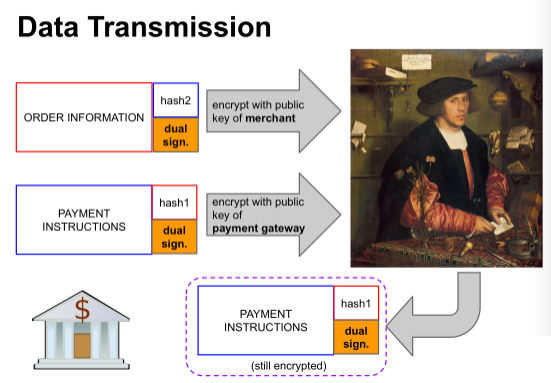
\includegraphics[width = \textwidth]{./images/SET.png}
				\end{figure}
				SET failed because the implementation was very difficult to put in place, and also not fully transaprent. The main problem was the requirement of a digital certificate \emph{also for the client}: let's say it's not the most scalable solution. 
				
			\subsubsection{HTTPS}
				HTTP over Secure Software Level is the de facto standard for the secured internet communication. SSL is the name for the previous versions of TLS (all TLS version behind 1.2 are deprecated at this time).\\
				TLS (the actual securing protocol) redesigns the classic HTTP handshake, adding the "secure suit selection" part: this first part is issued by the client, that at first connections \emph{tells the server which are his preferences for}
				\begin{itemize}
					\item key exchange algorithm
					\item bulk encryption algorithm
					\item message authetication code algorithm
					\item random number generation function used
				\end{itemize}
				At every voice in the cipher suit is associated a preference level, and the server sends back the configuration of algorithms to use for the communication basing his decision on this preference level. In the server response it also sends his certificates. \emph{TLS also supports client authentication}, so it allows the client to reply with his own certificate set. The handshake can be summarized as so:
				\begin{figure}[H]
					\centering
					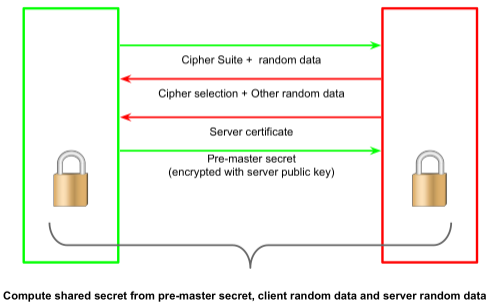
\includegraphics[width = \textwidth]{./images/TLS.png}
				\end{figure}
				
				\paragraph{Man in the Middle Attacks}
					TLS is designed to be resistant to MitM attacks: what an attacker can do to impersonate the server is cut out from the handshake
					\begin{itemize}
						\item He cannot let the original server certificate go through, because he won't be able to be trusted
						\item He cannot send a fake certificate, the client can easily notice
					\end{itemize}
	
	\clearpage \part{Secure Network Architecture}
		\section{Firewalls}
			Firewalls are network access control systems that verify all the packets flowing through them. Easy. This verification can be don at IP level (like Access Control Lists) or at transport layer (NAT level, to be precise).
			
			\paragraph{Firewall Cons}
				Firewalls are perfect to filter traffic, but firewall positioning is a problem \emph{by itself}: a FW is totally useless if an attacker can go around it. Also, the firewall is usually a computer by itself: they're vulnerable by itself and can be cracked, put offline etc. Moreover, the configurability of the firewall renders it a victim of bad configuration issues: if we're adding the wrong rules we're restricting too much OR not restricting enough the network we're rying to protect.
				
			\subsection{Firewall Taxonomy}
				\paragraph{Network Layer Firewall}
					We can divide network layer firewalls in
					\begin{itemize}
						\item ACL. They just filter packets basing on static rules on the address or port, for example. ACL are very limited when it comes to detect attack that spans over multiple packets: they're old. They can perform only a static analysis that spans in detail up to the IP options enabled, and not fully even to TCP or UDP. 
						\item Stateful packet filter firewalls. This kind of packet filters are an evolution of ACL, with added state: a stateful packet filter knows if a packet is in some way \emph{related} with the previous or the next one. These firewalls are much more powerful wrt ACL: the ability to detect exploits \emph{across packets} enables them to track connections and validate them. Also, \emph{there's almost no need for reflexive rules\footnote{response rules}}, because the state encapsulates it. Firewalls of this kind would alterthe ISN of TCP sessions in order to make more difficult to exploit a TCP packet for an attack, an will set "tolerance timers" on top of stateless protols (UDP) that simulates the "acceptance window" for a safe packet.
					\end{itemize} 
				
				\paragraph{Application Layer Firewall}
					At application level we can encounter
					\begin{itemize}
						\item Circuit level firewalls (legacy stuff). They act as a TCP level proxy.
						\item Application proxies: circuit level firewalls, but on top of the stack. They're not transparent to the client: the connection should pass through the proxy every time, to inspect/verify/sanitize it. 
					\end{itemize}
		
		\section{Architectures for Secure Networks}
			\subsection{Multi Zone Architectures}
				"Multi zone architectures" is the boring name for the \emph{castle approach} to network design; this relies on the assumption that all that's inside is good, all that's outside is harmful. However, the limit of this approach are evident: how can I safely allow external access to my network? Well, we can simply \emph{sectorize our internal citadel} into partitions that differs in the \emph{level of clearance needed to access}.\\
				The classic multi zone architecture is divided in:
				\begin{enumerate}
					\item the internet
					\item a tunnel of DMZs (demilitarized zone) that's an intermediate portion of the network: this partition is \emph{reachable from the public} and so all the machines in this zone \emph{should not be trusted}. We can put several of them "in series" between th einside and the outside
					\item an internal private network (that can be furtherly divided)
				\end{enumerate}
				ALL THESE LEVEL ARE SEPARATED BY DIFFERENT FIREWALLS that are configured in different ways.
				
			\subsection{Virtual Private Network}
				VPNs are a threath to pure castle-approach structured networks. They in fact open a tunnel through them.
				
				\paragraph{Full Tunnelling}
					ALL traffic generated by a VPN connected host pass through the local area network of the organization, allowing him to benefit of the internal resources (among the others: the \emph{firewall}).
				
				\paragraph{Split Tunnelling}
					"Local" traffic is redirected inside the organization's LAN, while the Internet traffic is left to the ISP to carry out. This actually open a door on a LAN. This modality is the most dangerous to a network that relies on a castled approach. 
	
	\clearpage \part{Malicious Software}
		\section{Malwares}
			What are malwares? Mal(icious soft)wares are \emph{programs that are explicitly written to violate a security policy} or more in general, \emph{harm a system}.
			
			\subsection{Categories of Malwares}
				Malwares can have several features and objectives. We can classify them basing on these traits:
				\begin{itemize}
					\item Viruses: self propagating piece of code
					\item Worms: self propagating \emph{program}
					\item Trojans: virus "in disguise"
				\end{itemize}
				Computer viruses were first created as a proof of concept for programs that auto replicate or modifies on their own. The security problem was understood later. An interesting theoretica result is the formal impossibility to build a perfect virus detector: this problem can be seen as a formulation of the halting problem (still undecible while I'm writing). 
				
		\section{Lifecycle of a Malware}
			The life of a malware is divided in 4 main stages:
			
			\paragraph{Reproduce and Infect}
				In these first two phases the malware is reproducing the logic under it and must not be detected. The tradeoff here is infection speed (or broad) vs detection probability. Nowadays, the spreading vector is something not necessarily hidden in the code, but more a known vulnerability or a social engineering attack. Several infection techniques are used: some viruses hides in the master boot record of computers or in the boot partitions. Or simply modify neighbouring files (like multicavity viruses, that inject code in unused region of program code).\\
				Another method is hiding in a macro: an innocent like document can transform in a weapon if a macro is inserted (and blindly executed). 
				
			\paragraph{Hide}
				More than a phase, a \emph{condition}: as already mentioned, being hidden equals not being detected, that's fundamental for a malware. There are plenty of techniques to stay hidden: hiding in macros, being polyglot etc. 
				
			\paragraph{Deliver Payload}
				Well: deliver payload. Take a bunch of harmful code and execute it where the virus had reached. 
	
		\section{Defending from a Malware}
			Malwares are a problem. They can harm everything related to software, from the hardware itself, to communications, to assets, to public images. Defending against them is necessary: we see three main approaches.
			\begin{itemize}
				\item Software maintainance: often viruses exploits known software vulnerabilities. Patching them (and updating the softwares in general) makes the environment less exploitable from an attacker
				\item Malware signatures: so far one of the most utilized techniques to recognize malicious software. A program can be "recognized" from his signature (usually an hash derived from his bytecode). This enables antivirus to detect malicious softwares and block them.
				\item Behavioral and static executable analysis: viruses can worms can be recognized also by "known bad software practices" that are usually exploited, like the utilization of some known vulnerable library or the exhibition of a suspicious behaviour at runtime
			\end{itemize}
			
			\subsection{Known Malicious Behaviours}
				Not all (known) patterns of execution of malwares are easily detectable or static:
				\begin{itemize}
					\item A program can be polymorphic or metamorphic, so be able to modify itself at runtime (for example inserting random dead code or on the fly code reordering). More specifically, we tlak about "software polymorphism" when the syntax and the overall code of the malware change during execution, but the semantic remains the same. If encryption is used to do so, then the technique called \emph{packing} is being used. Instead, metamorphism alters the behaviour of the program \emph{in an ineffective way}, so that the final result is achieved nonetheless. Techniques to metamorph a piece of code are inserting no-operation or useless always verified checks, or to scramble the execution flow without altering the algorithm. 
					\item A malware can be dormant, and waiting for particular conditions to be met: a particular time, a trigger...
					\item Anti virtualization technique can be deployed: a program could \emph{detect} when it's being debugged and change his behaviour
					\item Rootkits: rootkits defines an approach to hacking a machine. A rootkit is a set of tool that "implants a root user" on a machine. This root user can then use other pieces of the rootkit itself to harm the system itself. I like more the Wikipedia definition though\footnote{\emph{A rootkit is a collection of computer software, typically malicious, designed to enable access to a computer or an area of its software that is not otherwise allowed (for example, to an unauthorized user) and often masks its existence or the existence of other software.}}.
				\end{itemize}
				
				\paragraph{Rootkits}
					Philosophy at the base of the rootkit: "become root and use your toolkit to remain so". Rootkits are collections of softwares, that each helps in a task (like becoming root, hiding processes and srevices). The "hiding services and processes" part is crucial: to avoid being detected, hiding malicious processes (and the tracks left behind in general) is fundamental.\\
					Rootkits are divided in two macro categories:
					\begin{itemize}
						\item Userland rootkits, that exploits userspace tools (like normal OS utilities) to remain hidden and gain accesses and priviledges.
						\item Kernel space rootkits, which instead are executed at kernel level. They're much more difficult to build and implant (as they require several high level authentication in order to do so) but they're also much more powerful. Kernel space rootkits can be detected only after \emph{post mortem analysis}. The kernel space rootkits, operating at (and under) OS level can completely hide software artifacts, but also \emph{compromise the system} in a significative way. They can even intercept and redirect syscalls.
					\end{itemize}
					At a higher level of technicality, Bootkits (rootkits hidden in the master boot record or in the boot artition) and HyperVisor level rootkits exists. 
	
	\clearpage \part{Mobile Security}
		\section{Mobile Devices}
			Why should an attacker target mobile devices? Here's a bunch of pros:
			\begin{enumerate}
				\item Always online
				\item Nowadays, high computing capability
				\item Handles sensitive data
			\end{enumerate}
			So harming a person mobile device means that the attacker gains access to private emails and messages, maybe private accounts or personal transactions, and can be sure that a "way out" on the network is always present. This makes mobile devices extremely attractive for hackers.
			
		\section{Security Models for Mobile Operative Systems}
			\subsection{Apple Model}
				Apple mobile operative system iOS implements code signing to enforce security. This method asks developers to digitally sign (usually through a checksum verifier method) the code and the whole app is verified \emph{every time it's executed}. The certificate is signed by Apple Store, that is the only trusted element of the Apple ecosystem. \emph{No unsigned code can be executed in an Apple device.}\footnote{Unless jailbreak.}\\
				Another measure deployed is sandboxing with predefined permissions: the apps developed targeting apple iOS have no access to \emph{any} file or hardware in the device; they can only access their "personal" directory. The kernel uses Mandatory Access Control to manage accesses.
			
			\subsection{Android Model}
				Android checks the \emph{integrity} of the cryptographic sign of the app at installing time, but not during runtime. This allows the app to put in place dynamic code generation, or OTA silent updates. Also, every app can be \emph{self signed} and there's no CA to regulate that.\\
				Also Android sandboxes apps, but the permissions are handled by the underlying linux kernel.
			
	\clearpage \part{Exercises tips and notes}
		\section{Binary Exploits}
			\subsection{Buffer Overflows}
				For buffer overflows, we need to keep in mind how the stack is organized when a function is called. When function F calls functions D, in order, we have\footnote{in the reference architecture, so a GCC compiled C code with target a 32 bit machine, with all the options for debug and security disabled}:
				\begin{enumerate}
					\item Arguments in reverse order
					\item The instruction pointer of F
					\item The base pointer of F (this address will be the new base pointer)
					\item The local variables of D:
						\begin{itemize}
							\item if standard types, in order
							\item if structs, the field are allocated in reverse order
							\item if vectors, allocated from the last element
						\end{itemize}
				\end{enumerate}
				Remember: \emph{stack grows towards smaller addresses}.\\
				Also, watch out for the dimension of the exploit: if the shellcode/malicious code is bigger than the available space on the stack, it means that the only technique we can use is return to libc (or at least exploiting some sort of enviromental variable). 
				
				\paragraph{Building the exploit}
					To exploit a buffer overflow vulnerability, we need to
					\begin{enumerate}
						\item Identify which variables we can control
						\item Find the one initialized without check
						\item Calculate how many bytes we have to overwrite in order to modify the return address of the function
						\item Using this information to substitute the saved return address with one "known", possibly insert a nop sled\footnote{A series of null operations (nop) to "nullify" a portion of memory.} to be sure
						\item The resulting exploit will 99\% look like a sequence of nop followed by the actual exploit and an address targeting somewhere in the nop sled
					\end{enumerate}
					Something to watch out: sometimes this string must contain a certain type of parameter, so watch out for other controls!
				
				\paragraph{Constants}
					In the referenced architecture, these are the usual values for the system variable types / general dimensions
					
					\begin{center}
						\begin{tabular}{ |c|c|c|}
							\hline
							Type & Size in bits & Size in bytes \\
							\hline
							\hline
							Word (memory location length) & 32 & 4\\
							Pointer (and registers) & 32 & 4 \\
							Integer & 32 & 4 \\
							Char & 8 & 1 \\
							Structs & (sum of bits of fields) & (sum of bytes of fields)\\
							\hline 
						\end{tabular}
					\end{center}
					
			\subsection{Format String}
				How to write an exploit for a format string vulnerability, let's directly focus on what to do if we want to write an entire \verb|DWORD|, and not a single 16-bit \verb|WORD|\footnote{Why? Because we can, \textit{sir}.}.\\
				We need:
				\begin{enumerate}
					\item Some malicious data (32 bit of data)
					\item A place where we want to write such data
					\item A stack offset where \textit{we know} we can put data; we will put the target address
				\end{enumerate}
				We build the exploit this way:
				\begin{enumerate}
					\item The two target addresses
						\begin{itemize}
							\item If the first half of the payload is \emph{greater than}\footnote{in decimal} the second one, then we write the address and the address plus two in order in the string (with the usual format for hexadecimal values: \textbackslash \verb|0A|)
							\item If not, we reverse them: first we put \verb|ADDR + 2| then \verb|ADDR|
						\end{itemize}
					\item the first character placeholder \%Nc where 
						\begin{equation}
							N = decimal(lower\, part\, of\, payload) - \#(characters\, already\, written)
						\end{equation}
					\item the first \%N\$hn placeholder to instruct to write, where N is the displacement in the stack where we found out our string with the address would be. WATCH OUT: the displacement can depend from the lenght of the string we're passing!
					\item second character placeholder, this time
						\begin{equation}
							N = decimal(higher\, part\, of\, payload) - decimal(lower\, part)
						\end{equation}
					\item the second and last \%N\$hn placeholder (the one that effectively write), where N is the offset we calculated in (3) incremented by one
				\end{enumerate}
		\section{Web Vulnerabilities}
			\subsection{Cross Site Scripting}
				It's important to recognize the XSS vulenrrability we're working with. Here's a list of signals you can look after for each XSS vulns we've seen
				\begin{center}
					\begin{tabular}{ | m{5cm} || m{5em} | m{5em} | m{5em} |}
						\hline
						Type of error & Stored XSS & Reflected XSS & DOM-Based XSS \\
						\hline
						\hline
						Unchecked insertion of data in the database & X & & \\
						\hline
						Unchecked write of content to the client \emph{from DB} & X & & \\
						\hline
						Unchecked write of content to the client \emph{from client itself} & & X & X \\
						\hline
						Unchecked write of content to the client \emph{using a client side technology} & & & X \\
						\hline
						\textbf{Type of remedy} & Input sanitizing, server side, CSP & DB check of entities & Client side sanitizing \\ 
						\hline
					\end{tabular}
				\end{center}
				
			\subsection{Cross Site Request Forgery}
				In order to have a CSRF, some conditions are necessary:
				\begin{enumerate}
					\item cookies used somewhere
					\item state changing actions
					\item "automation" of user interaction through ambient variables (usually cookies, or sessionstorage)
				\end{enumerate}
				What to remember for a valid CSRF attack: it \emph{99\% of the cases} involves 3 parties: these are the attacker, a \emph{target website} and the client.
				
			\subsection{SQL Injection}
				To spot an SQL injection type of vulnerability is enough to see if there's some unchecked insertion in the database, some unsanitized input. Usually the countermeasures used are
				\begin{itemize}
					\item SQL prepared statements, that converts all inputs to string
					\item Client side input sanitizing (easily disabled)
					\item Server side input sanitizing 
				\end{itemize}
				This kind of attacks usually require to extract some information from a DB; an SQLi injection exploit follows a rigid structure
				\begin{enumerate}
					\item a string terminator (apice or double apices) that is used to close the parameter that can be exploited
					\item either a modified or additional condition to manipulate a \verb|WHERE| clause, where usually the parameters are inserted
					\item either a 
						\begin{itemize}
							\item query terminator plus comment symbol
							\item UNION clause
							\item apices (in the case we'd like to still use the part of the original query we've cut out)
						\end{itemize}
				\end{enumerate}
				If the injected code exploits a vulnerability in a \verb|INSERT INTO| clause, the additional condition of the list is replaced with an additional \verb|VALUES| clause.\\
				REMEMBER: the malicious input should not undergo transformations that alter the payload (like base64 encoding or hashing of some kind). So WATCH OUT for this kind of encodings. Also, while building the exploit, remember that the data we've to verify that the data were correctly inserted OR we must be able to exfiltrate properly the information we're trying to steal. \emph{This is not obvious} and can require several logical steps to get to the right infos.
				
		\section{Secure Network Architectures}
			\subsection{Designing a Secure Network Architecture}
				Quick list of things to keep in mind when positioning firewalls to divide subnets:
				\begin{itemize}
					\item 99\% of networks needs a DMZ. Things that go in a DMZ:
						\begin{itemize}
							\item The web server ($\Leftrightarrow$ the company must be accessible through a website)
							\item A mail server (but only the inbound one, the InSMTP one. There's no need for an outbound mail server to be placed in the DMZ)
							\item \textbf{The Proxy}: if the network requires some traffic to go through a proxy machine, it's 99\% of the time placed \textit{outside} the main LAN $\rightarrow$ in the DMZ
							\item A DNS server: this can be placed either inside the LAN or the DMZ. It makes more sense in the DMZ though
						\end{itemize}
						Things that \textbf{DO NOT} go in a DMZ:
						\begin{itemize}
							\item The outbound mail server 
							\item The application server: in most cases, services are provided through the web $\rightarrow$ the application server with all the application logic must not be exposed, but must be accessible from the web server
							\item The database. No need to say why putting the DB in the DMZ is a bad idea
						\end{itemize}
					\item It's usually a good practice to separate "logically different" areas of the network\footnote{also for congestion reasons}: in the seen exercises, behind the DMZ, usually the LAN is partitioned in:
						\begin{itemize}
							\item A \textit{service} segment where the application server resides, alongside the DB and eventually a mail server
							\item A \textit{lan} segment
							\item An additional \textit{special purpose} segment if needed (to manage an IoT sensor swarm, a pool of machine, or simply a different sector in the organization)
						\end{itemize}
					\item Edges of network segments are \textit{firewalled}
					\item Multiple segments can use the same firewall, but it's not impossible to have three or more deep chains of firewall to further partition the overall network
				\end{itemize}

			\subsection{ACLs and Firewall Rules}
				Classic approach to firewall rules in general:
				\begin{enumerate}
					\item deny all
					\item allow selected
					\item (additional) add reflection rules to allow symmetric communication
				\end{enumerate}
				Typical exercise has this table to fill out (here with some rule example):
				\begin{center}
					\begin{tabular}{ | m{3em} | m{2em} | m{2em} | m{4em} | m{2em} | m{2em} | m{5em} | m{5em} |}
						\hline
						Firewall ID & SRC IP & SRC port & direction & DST IP & DST port & policy & description\\
						\hline
						\hline
						FW1 & any & any & net1 $\rightarrow$ net2 & any & any & deny & deny all incoming\\
						\hline
						FW1 & any & any & net1 $\rightarrow$ net2 & any & any & deny & deny all outgoing\\
						\hline
						FW1 & any & any & net1 $\rightarrow$ net2 & any & 80 & allow & allow web traffic\\
						\hline
						FW1 & any & 80 & net2 $\rightarrow$ net1 & any & any & allow & allow web traffic, response rule to previous \emph{only for stateless fws}\\
						\hline
						&&&&&&&\\
						\hline
						&&&&&&&\\
						\hline
					\end{tabular}
				\end{center}
				REMEMBER: the specified port for a protocol is one you \emph{receive} on.
				
		\section{Malwares}
			Typical exercise on this part: recognize which techniques is being used by a program to hide. Quick list of easy-to-prove properties:
			\begin{center}
				\begin{tabular}{ | m{10em} || m{6em} | m{4em} | m{6em} | m{6em} |}
					\hline
					Property & Polymorphism & Packing & Metamorphism & Trigger based \\
					\hline
					\hline
					Same instructions, different order (jumps inserted) & & & X & \\
					\hline
					Different instructions & X & X & & \\
					\hline
					Encrypt decrypt primitives & X & X & & \\
					\hline
					Compression primitives & & X & & \\
					\hline
					Same syscalls & X & X & & \\
					\hline
					Lots of "sleep" functions accessed through conditional instructions on some hardware property & & & & X \\
					\hline
					\textbf{Best practice} & dynamic analys & dynamic analysis  & dynamic analysis & static analysis \\
					\hline
				\end{tabular}
			\end{center}
				
				
\end{document}
